%----------------------------------------------------------------------------
\section{Elektronika 1, 2}
{\footnotesize Passzív áramköri elemek tulajdonságai, RC és RLC hálózatok. Diszkrét félvezető eszközök, aktív áramköri elemek, alapkapcsolások. Integrált műveleti erősítők. Tápegységek. Mérőműszerek.}
%----------------------------------------------------------------------------
\subsection{Passzív áramköri elemek tulajdonságai, RC és RLC hálózatok.}
\paragraph{Ellenállás}
Jele: $R$\\
Kiszámítása: $R = \nicefrac{U}{I}$\\
Az ellenállás kapcsolata a teljesítménnyel: $P=\nicefrac{U^2}{R}\quad P=U \cdot I$\\
\begin{itemize}[nosep]
	\item Állandó értékű ellenállások
	\begin{itemize}[nosep]
		\item Felépítés: szigetelő hordozó, vezető réteg, fém kivezetések
		\item Főbb típusok: huzalellenállás, rétegellenállás, tömbellenállás
		\item Beszerelés: furatba, felületre (SMD)
		\item Értékét Ohm-ban [$\Omega$] adják meg  $\rightarrow R = \rho \cdot \nicefrac{l}{A}$ alapján
		\item Névleges érték, tűrés $\rightarrow$ nem tudják pontosan gyártani őket, ezért van egy tűréshatár \%-ban
		\item Terhelhetőség: Watt-ban, maximális teljesítménye; az ellenállás melegszik $\rightarrow$ hődisszipáció
		\item Ellenálláskódok $\rightarrow$ ellenálláson színkódok és számkódok
	\end{itemize}
	\item Változtatható ellenállások (potenciométerek)
	\begin{itemize}[nosep]
		\item Típusok: huzalpotenciométer, rétegpotenciométer
		\item Szabályozási jellemző: lineáris, nem lineáris (logaritmikus, fordított logaritmikus, S alakú)
		\item Terhelhetőség: a teljes névleges ellenállásra vonatkozik, az ebből számított áramot a csúszka egyik állásában sem haladhatja meg a potenciométer árama $$I_{\max} = \sqrt{\frac{P}{R_\text{névleges}}}$$
	\end{itemize}
	\item Speciális ellenállások (PTK, NTK, VDR)
\end{itemize}

\paragraph{Kondenzátor}
Jele: $C$\\
Kiszámítása: $Q = C \cdot U$\\
Mértékegysége: $\nicefrac{As}{V} =$ Farad
\begin{itemize}[nosep]
	\item Állandó kapacitású kondenzátorok
	\begin{itemize}[nosep]
		\item Felépítés: fém fegyverzetek, fém kivezetések, dielektrikum
		\item Főbb típusok: sík, hengeres, tekercselt, többrétegű
	\end{itemize}
	\item Változtatható kondenzátorok
	\begin{itemize}[nosep]
		\item Felépítés: mozgatható fegyverzetek, légrés (a fegyverzetek alakja határozza meg a szabályozási jelleget)
	\end{itemize}
\end{itemize}

\paragraph{Tekercs}
Jele: L\\
Kiszámítása: $B = \nicefrac{\Phi}{A}$\\
\begin{description}[nosep]
	\item[Indukció] a tekercsben feszültség jön létre, ha a tekercsen átmenő fluxus megváltozik.
	\item[Önindukció] feszültség indukálódik a tekercsben akkor is, ha a fluxus változását áramának megváltoztatásával saját maga idézte elő.
\end{description}
\textbf{A feszültség azért jön létre, mert megváltozik az áram folyásának iránya, mert ilyenkor a fluxus is megváltozik.}

\paragraph{Transzformátor}
Magyar találmány: Bláthy-Zipernowsky-Déry. Zárt vasmag, két oldal: primer és szekunder tekercs. $$ \frac{U_1}{U_2} = \frac{N_1}{N_2}$$
ahol $N$ a tekercs menetszáma.\\
Felhasználás: igény szerinti feszültség előállítás a 230V-os hálózati feszültségből és a villamos energia gazdaságos szállítása.

\subsubsection{RC és RLC hálózatok}
\paragraph{Soros RC hálózat} esetén az \emph{áramerősség} a közös mennyiség. A feszültségvektorok diagramjából impedancia háromszöget kapunk, melyből Z kiszámíthatjuk a $Z$ impedanciát:
$$Z^2 = R^2 + X_c^2 \rightarrow Z = \sqrt{R^2 + X_c^2}$$
$X_c$-vel a kondenzátor reaktanciája.
A kapcsolás kis frekvencián $X_c$ miatt szakadásként, nagy frekvencián vezetőként, ohmos ellenállásként viselkedik. Határfrekvenciának ($f_h$) nevezzük az áramkörben folyó váltakozó áram azon frekvenciáját, melynél $ R = X_c$.
\begin{figure}[h]
	\centering
	\begin{subfigure}[b]{0.45\textwidth}
		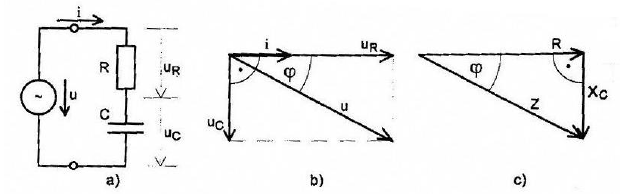
\includegraphics[width=\linewidth]{fig/10-serialRC_Schematic}
		\caption{Soros R-C kapcsolás és vektor diagramja}
		\label{fig:10-serialrcschematic}
	\end{subfigure}
	\begin{subfigure}[b]{0.45\textwidth}
		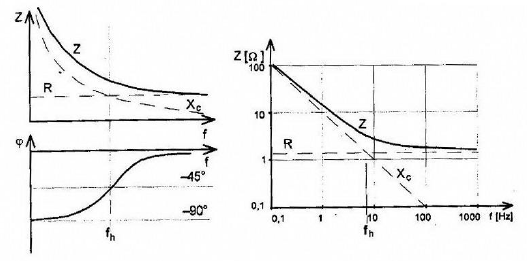
\includegraphics[width=\linewidth]{fig/10-serialRC_Plot}
		\caption{Soros R-C áramkör impedanciájának és fázisszögének változása}
		\label{fig:10-serialrcplot}
	\end{subfigure}
\end{figure}


\paragraph{Párhuzamos RC} hálózatnál a \emph{feszültség} a közös mennyiség. Az áramok vektorainak diagramjából admittancia (Y) háromszöget kapunk:
$$Y^2 = G^2 + B_c^2 \rightarrow Z = \sqrt{G^2 + B_c^2}$$
ahol $B_c = \nicefrac{I_c}{U}$ és $G=\nicefrac{I_R}{U}$.
A kapcsolás kis frekvencián $X_c$ miatt ohmos ellenállásként, nagy frekvencián rövidzárként ($0\Omega$ os ellenállásként) viselkedik. A határfrekvenciát ugyan úgy határozhatjuk meg, mint a soros RC hálózatok esetében.
\begin{figure}[h]
	\centering
	\begin{subfigure}[b]{0.45\textwidth}
		\centering
		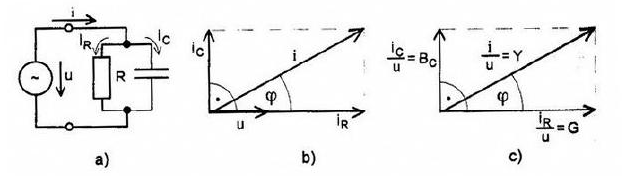
\includegraphics[width=\linewidth]{fig/10-parallelRC_Schematic}
		\caption{Párhuzamos R-C kapcsolás és vektor diagramja}
		\label{fig:10-parallelrcschematic}
	\end{subfigure}
	\begin{subfigure}[b]{0.45\textwidth}
		\centering
		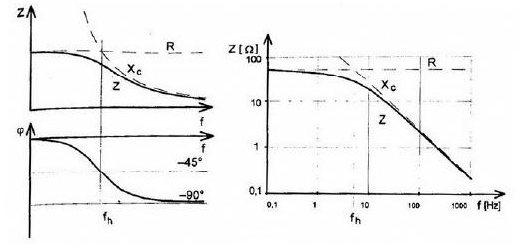
\includegraphics[width=\linewidth]{fig/10-parallelRC_Plot}
		\caption{Párhuzamos R-C áramkör impedanciájának és fázisszögének változása}
		\label{fig:10-parallelrcplot}
	\end{subfigure}
\end{figure}

\paragraph{Soros RLC} Másnéven \emph{sávzáró szűrő}. A soros kapcsolás miatt mindegyik elemen ugyanaz az I áram folyik át, tehát az \emph{áramerősség a közös mennyiség}. Az impedancia háromszög alalpján:
$$ Z = \sqrt{R^2 + (X_L - X_C)^2}$$
ahol $X_L$ és $X_C$ a tekrecs, ill. a kondenzátor reaktanciája.
\begin{figure}[h]
	\centering
	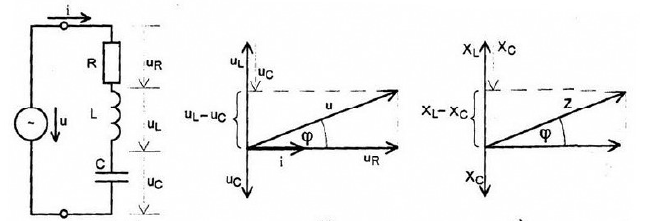
\includegraphics[width=0.5\linewidth]{fig/10-serialRLC}
	\caption{Soros R-L-C kapcsolás és vektor diagramja}
	\label{fig:10-serialrlc}
\end{figure}

\paragraph{Párhuzamos RLC} Másnéven \emph{sáváteresztő szűrő}. Itt a \emph{feszültség} a közös mennyiség. Minden áramot ($I_R, I_L, I_C$) a közös feszültséggel osztva admittancia háromszöget kapunk, melynek alapján:
$$ Y = \sqrt{G^2 + (B_L - B_C)^2}$$
\begin{figure}[h]
	\centering
	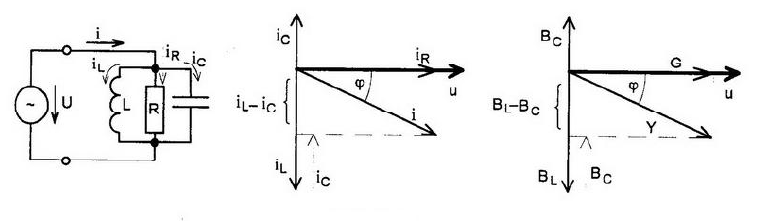
\includegraphics[width=0.5\linewidth]{fig/10-parallelRLC}
	\caption{Párhuzamos R-L-C kapcsolás és vektor diagramja}
	\label{fig:10-parallelrlc}
\end{figure}


\subsection{Diszkrét félvezető eszközök, aktív áramköri elemek, alapkapcsolások.}
\subsubsection{Dióda}
\emph{Egy P és Egy N réteget tartalmaz}. Jelölése kapcsolási rajzon: 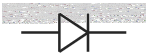
\includegraphics[width=0.2\linewidth]{fig/10-diode}

Működését egyszerűen jellemezhetjük: az egyik irányban engedi folyni az áramot, a másik irányban nem. A jelölés szerint a háromszög irányában folyhat az áram, visszafelé nem. Felhasználásának legáltalánosabb módja az \emph{egyenirányítás}.

A dióda legfőbb jellemzői:
\begin{itemize}[nosep]
	\item rajta átfolyó maximális áramerősség
	\item rajta eső feszültség 
	\item felhasználási terület
\end{itemize}
A diódák általában henger alakúak, két kivezetésük a henger két véglapján található, a rajta levő jelzés alapján megállapíthatjuk melyik vezeték a katód. A diódán az áram az anód irányából a katód irányába folyik (nyitó irányú kapcsolás). Záró irányú kapcsolás esetén elenyészően kicsi áram folyik keresztül a diódán.

A dióda működőképességét ellenállásmérő műszerrel ellenőrizhetjük a következőképpen: mindkét irányban megmérjük az ellenállását. Ha azt tapasztaljuk, hogy az egyik irányban mutat valamekkora ellenállást, a másikban pedig közel végtelen ellenállású akkor a dióda működőképes. A félvezetőkben a szabad töltéshordozók száma és anyag vezetőképessége a hőmérséklettel arányosan változik. Félvezető tulajdonsággal rendelkeznek az alábbi anyagok nagy tisztaságban: germánium (Ge), szilícium (Si), szelén (Se), valamint néhány vegyület: galliumarzenid (GaAs), indiumfoszfid (InP) stb. Nyitóirányú és záróirányú feszültség.(???)%TODO

\paragraph{Zener-dióda}
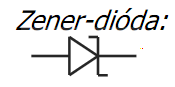
\includegraphics[width=0.2\linewidth]{fig/10-zener-diode}\\
Stabilizál. Adott nagyságú záróirányú feszültségnél hirtelen megnő a félvezető dióda árama. Konstrukciótól függően különböző letörési feszültségek vannak
\paragraph{Schottky dióda} nagyon gyorsan nyitó/záró dióda típus. Tápegységekben gyakran találkozunk velük.

\subsubsection{Alapkapcsolások}
\begin{theorem}[Kirchhoff I. törvénye]
	Egy csomópontba befolyó áramok összege megegyezik az onnan elfolyó áramok összegével. (csomóponti törvény) $$ \Sigma I = I_1 + I_2 + I_3 + \dots$$
\end{theorem}

\begin{theorem}[Kirchhoff II. törvénye]
	Bármely zárt hurokban az áramköri elemeken lévő feszültségek előjel helyesen vett összege nulla. (hurok törvény) $$ \Sigma U = 0 $$
\end{theorem}

\paragraph{Soros kapcsolás}
Soros kapcsolásban ugyanaz az áram folyik át minden ellenálláson, a feszültségek
összeadódnak. A sorosan kapcsolt ellenállások eredőjét az ellenállások összegzésével kapjuk, így az eredő nagyobb lesz bármely elem értékénél.
$$R_e = R_1 + R_2 + R_3\quad 
L_e = L_1 + L_2 + L_3\quad 
\frac{1}{C_e} = \frac{1}{C_1} + \frac{1}{C_2} + \frac{1}{C_3}$$

\paragraph{Párhuzamos kapcsolás}
Párhuzamos kapcsolásban azonos feszültség lép fel minden ellenálláson, az áramerősségek pedig összeadódnak. A párhuzamosan kapcsolt ellenállások eredőjét az ellenállások reciprokának összegével képezzük, ami még nem az eredőt,hanem annak a reciprokát adja ezért ennek is venni kell még a reciprokát.
$$\frac{1}{R_e} = \frac{1}{R_1} + \frac{1}{R_2} + \frac{1}{R_3}\quad \frac{1}{L_e} = \frac{1}{L_1} + \frac{1}{L_2} + \frac{1}{L_3}\quad 
C_e = C_1 + C_2 + C_3$$
%Párhuzamosan kapcsolt ellenállások, induktivitások, illetve sorosan kapcsolt kapacitások eredőjének kiszámításához használt speciális matematikai művelet a \emph{replusz}. Jele $\times$

\paragraph{Feszültségosztó}
Két ellenállás soros kapcsolása. A tápláló feszültség megoszlik az $R_1$ és $R_2$ ellenállás között. A feszültség az ellenállásokkal egyenes arányban oszlik meg.\\ %$$U_\text{ki}=\frac{R_2}{R_1 + R_2}$$
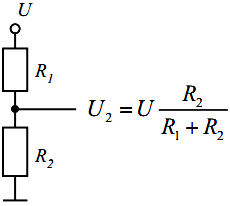
\includegraphics[width=0.25\linewidth]{fig/10-voltage_divider}

\paragraph{Wheatstone híd} A híd olyan négypólus, amelyben az áramköri elemek értékét úgy választjuk meg, hogy a kimeneti feszültség nulla legyen. Ezt nevezzük a híd kiegyenlített állapotának. A Wheatstone híd felhasználható ellenállás mérésre, mivel a szemben elhelyezkedő ellenállások szorzata = a másik két szemben lévő ellenállás szorzatával. Ha a négy ág közül három ismert, a negyedik kiszámítható. Kis áramok mérésére nem alkalmas.\\
%$$U_\text{ki} = 0\quad \text{ha}\quad R_1R_3 = R_2R_4 $$
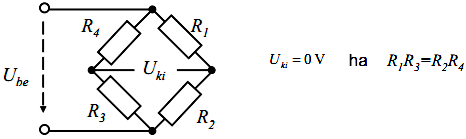
\includegraphics[width=0.5\linewidth]{fig/10-wheatstone_bridge}

\subsection{Integrált műveleti erősítők.}
A műveleti erősítő kiváló minőségű differenciálerősítő integrált áramkör, amely egyenfeszültség erősítésére is alkalmas. Analóg számítás- és szabályzástechnikai alkalmazásokhoz fejlesztették ki, de igen sokoldalúan alkalmazzuk őket.\\
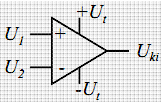
\includegraphics[width=0.25\linewidth]{fig/10-op_amp}\quad
Helyettesítő áramkör: 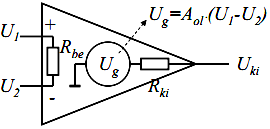
\includegraphics[width=0.5\linewidth]{fig/10-op_amp1}\\

Ideális műveleti erősítő jellemzői:
\begin{itemize}
	\item $U_\text{ki} =A_\text{ol} \cdot (U_1 - U_2)$
	\item Végtelen nagy nyílt hurkú feszültségerősítés ($A_\text{ol} = \infty$)
	\item Végtelen nagy bemeneti ellenállás ($R_\text{be} = \infty$)
	\item Zéró kimeneti ellenállás ($R_\text{ki} = 0$)
	\item Végtelen nagy sávszélesség: minden frekvencián ugyanakkora az erősítése
	\item Zéró ofszet (tökéletesen szimmetrikus felépítés): ha a bemeneti feszültségek megegyeznek, akkor a kimeneti feszültség zéró.
\end{itemize}

Valódi műveleti erősítők jellemző értékei:
\begin{itemize}
	\item szimmetrikus tápfeszültségre van szüksége (tipikusan $\pm 15V$)
	\item $A_\text{ol} \approx 10^5 \text{--} 10^6$
	\item $R_\text{be} \approx 1 \text{--} 200 M\Omega$ bipoláris bemenet, $R_\text{be} \approx 1000 \text{--} 2000 M\Omega$ FET bemenet
	\item $R_\text{ki} \approx 10 \Omega$
	\item $f_\text{min} \approx 0 Hz, f_\text{max} \approx ~\text{MHz}$
	\item közös módusú elnyomási tényező: $\text{CMRR} \approx 90 \text{--} 100 \text{dB}$
	\item véges kimeneti feszültségtartomány: $-U_t < U_\text{ki} < +U_t$
	\item véges maximális jelváltozási sebesség (slew rate): $\text{SR} \approx 0.5 \text{--} 30 \nicefrac{V}{\mu s}$
\end{itemize}

\paragraph{Negatív visszacsatolás} A kimeneti jel egy részét visszavezetik és kivonják a bemeneti jelből, így erősítésre ténylegesen a bejövő jel és az adott hányadban visszacsatolt kimeneti jel különbsége kerül. Így a kimenet megváltoztatása a negatív visszacsatolás révén ellene hat az U’ különbség növekedésének. Állandó bemeneti jel esetén a kimeneti feszültség is stabil értékre áll be. a negatív visszacsatolást alkalmazó áramköröknél a műveleti erősítő két bemeneti feszültségének különbsége a nagy nyílthurkú erősítés miatt igen kicsi.\\
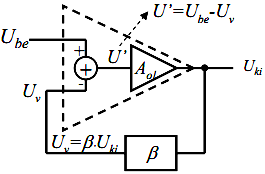
\includegraphics[width=0.5\linewidth]{fig/10-op_amp_neg_feedback}


\subsection{Tápegységek.}
\paragraph{Kapcsoló üzemű tápegységek} A korábban ismertetett tápegységek (hálózati transzformátor + egyenirányító + áteresztő tranzisztor) hatásfoka csak 25-50\%. Az áteresztő tranzisztor vesztesége jelentősen csökkenthető, ha kapcsolóval helyettesítjük. A transzformátor vesztesége (és mérete) pedig úgy csökkenthető, ha nagyfrekvenciás (20kHz-200kHz) váltakozó feszültséget transzformálnak.

A kapcsoló üzemű tápegységekben (switch-mode power supply (SMPS)) a feszültségszabályozást egy teljesítménytranzisztor változtatható kitöltési tényezővel történő egymást követő bekapcsolásával (teljes telítési állapot) és kikapcsolásával (lezárt állapot) valósítják meg. A terhelésnek megfelelő kitöltési tényezőjű gyorsan ismétlődő (10kHz\textendash100kHz) be- és kikapcsolás a szűrés után a kívánt nagyságú egyenfeszültséget biztosítja a kimeneten

A kapcsolóüzemű (feszültség csökkentő) tápegység működési elve: A K kapcsolót ciklikusan (T periódusidővel) kapcsolgatják: T\textsubscript{be} ideig az 1-es, T\textsubscript{ki} ideig a 2-es potícióba kapcsolják ($T=T be +T_\text{ki}$).

\subsection{Mérőműszerek.}
\begin{description}
	\item[Feszültségmérő] igen nagy belső ellenállású mérőműszer. Párhuzamosan kapcsolandó a mérendő alkatrésszel.
	\item[Áramerősségmérő] igen kis belső ellenállású mérőműszer, az áramkörbe sorosan kapcsolandó.
	\item[Digitális multiméter] Elsősorban egyenfeszültség, egyenáram, ellenállás és kapacitás mérésére használatos. Váltóáram és váltófeszültség effektív értékének mérésére is használható, de csak kisebb frekvenciákon.
	\item[Analóg multiméterek] elektronikus elven működő mérőműszerek,villamos mennyiségek mérésére alkalmasak, a mért mennyiség kijelzése analóg (pl. mutató) műszerrel történik.
	\item[Digitális multiméterek] többfunkciós mérőműszerek, a mért mennyiség számjegyes kijelzővel történik, ehhez mindegyik tartalmaz egy beépített A/D átalakítót és számkijelzőt.
	\item[Oszcilloszkóp] Mind feszültség, mind váltófeszültség mérésére alkalmas. A hagyományos analóg oszcilloszkóp képes megjeleníteni egy periodikus jel időbeli változását és így alkalmas a váltakozófeszültség olyan paramétereinek mérésére, mint pl. a periódusidő, felfutási idő, amplitúdó. Csak periodikus jeleket képesek stabil képpel megjeleníteni. A tárolófunkciós analóg oszcilloszkópok és a digitális oszcilloszkópok egyedi impulzusok megjelenítésére is alkalmasak.
	\item[Analóg oszcilloszkópok] Villamos jelek vizuális vizsgálatát teszi lehetővé egy katódsugárcsöves kijelző segítségével.
	\item[Digitális oszcilloszkópok] Villamos jelek vizuális vizsgálatát teszi lehetővé egy folyadékkristályos kijelző segítségével.
	\item[Szkópméterek] egy kétsugaras digitális tárolóoszcilloszkóp és egy digitális multiméter kombinációja, a mérési funkciók automatikusan a legjobb üzemi állapotra állítódnak be.
\end{description}